%%%%%%%%%%%%%%%%%%%%%%%%%%%%%%%%%% NOELIA %%%%%%%%%%%%%%%%%%%%%%%%%%%%%%%%%%

\section{Classical Controller Design}

%%%%%%%%%%%%%%%%%
\subsection{SISO Block Diagram}
\begin{frame}{Classical Controller Design}{SISO Block Diagram}	
	\begin{figure}
		\begin{tikzpicture}[ auto,
thick,                         %<--setting line style
node distance=1.5cm,             %<--setting default node distance
scale=0.75,                     %<--|these two scale the whole thing
every node/.style={scale=0.62}, %<  |(always change both)
>=triangle 45 ]

%-- Blocks creation --%
\draw
% DIRECT TERM %
node[shape=coordinate][](input1) at (0,0){}
node[shape=coordinate][](feed) at (0.5,0){}
node(sum1) at (2,0) [sum] {$\sum$}
node(controller) at (4,0) [block]{\Large $D(s)$}
node(plant) at (6,0) [block]{\Large $G(s)$}
node[shape=coordinate][](DummyNode) at (5,-1.5){}
node[shape=coordinate][](FeedbackNode) at (7.5,0){}
;

%-- Block linking --%
% INPUT %
\draw[-](input1)        -- node{\Large $U(s)$}(feed);
\draw[->](feed)  -- (sum1);

% OUTPUT %
\draw[-](plant)  -- (FeedbackNode);
\draw[->](FeedbackNode)       -- node {\Large $Y(s)$} (9,0);

% DIRECT TERM %
\draw[->] (sum1)            -- (controller);
\draw[->] (controller)       -- (plant);

% FEEDBACKS %
\draw[-] (FeedbackNode)  |- (DummyNode);
\draw[->] (DummyNode)  -| (sum1);

%-- Nodes --%
\draw%--------------------------------------------------------------
node at (input1)            [shift={(-0.04, -0.05 )}] {\Large \textbullet}
node at (FeedbackNode)      [shift={(0, -0.07 )}] {\Large \textbullet}
;
%-- Summation signs --%
\draw%--------------------------------------------------------------
node at (sum1) [right = -6.6mm, below = .6mm] {$+$}
node at (sum1) [right = -3mm, below = 3.9mm]  {$-$}
;

\end{tikzpicture} 
	\end{figure}
	\begin{itemize}
		\item U(s) refers to the desired angular position of the frame
		\item Y(s) is the actual angular position of the frame
	\end{itemize}
\end{frame}

%%%%%%%%%%%%%%%%%
\subsection{Stability Analysis}
\begin{frame}{Classical Controller Design}{Stability Analysis}	 
\begin{itemize}
	\item Nyquist plot
\end{itemize}
\begin{figure}
	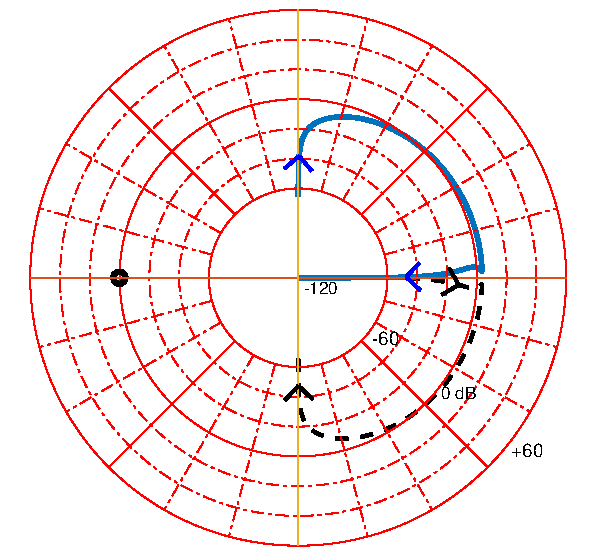
\includegraphics[scale=.5]{Pictures/nyquistCubli}
	\centering
\end{figure}	
\begin{displaymath}
	\si{Z_{RHP}\ =\ N\ +\ P_{RHP}} \nonumber
\end{displaymath}
\end{frame}

%%%%%%%%%%%%%%%%%
\begin{frame}{Classical Controller Design}{Stability Analysis}	
\begin{itemize}
	\item Root Locus
\end{itemize}
\begin{minipage}{\linewidth}
	\begin{minipage}{0.45\linewidth}
		\begin{figure}
			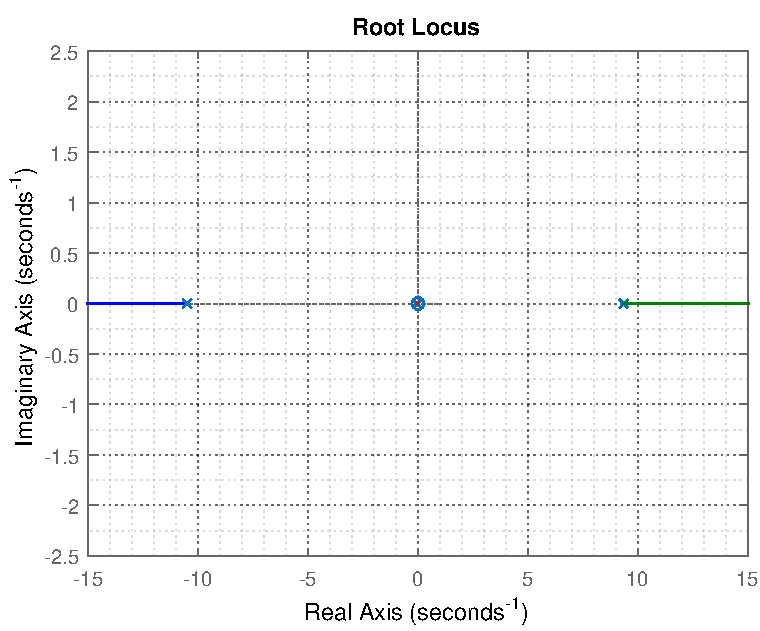
\includegraphics[scale=.42]{Pictures/rlocusCubli}
			\centering
		\end{figure}
	\end{minipage}
	\hspace{0.1\linewidth}
	\begin{minipage}{0.45\linewidth}
		\begin{figure}[H]
			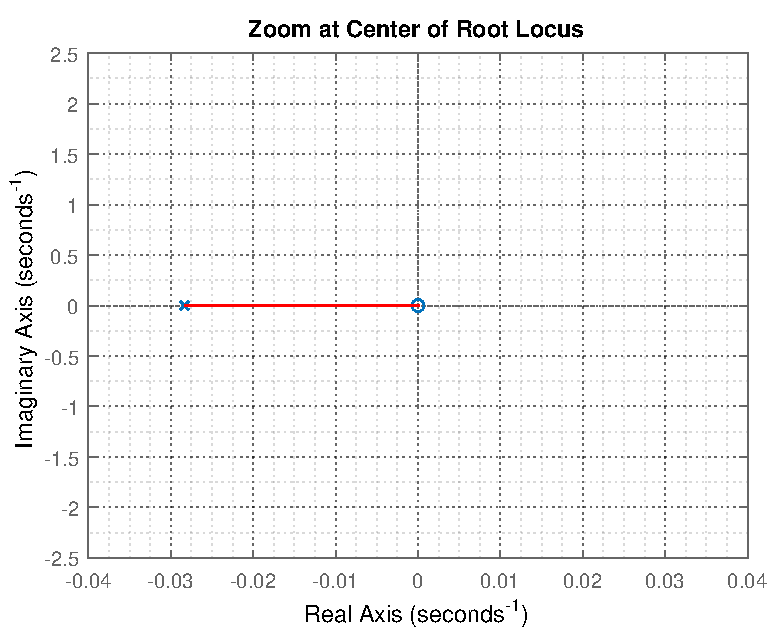
\includegraphics[scale=.35]{Pictures/rlocusCubliZoom}
			\centering
		\end{figure}
	\end{minipage}
\end{minipage}
\end{frame}

%%%%%%%%%%%%%%%%%
\subsection{Root Locus Design}
\begin{frame}{Classical Controller Design}{Root Locus Design}	
	\begin{figure}
	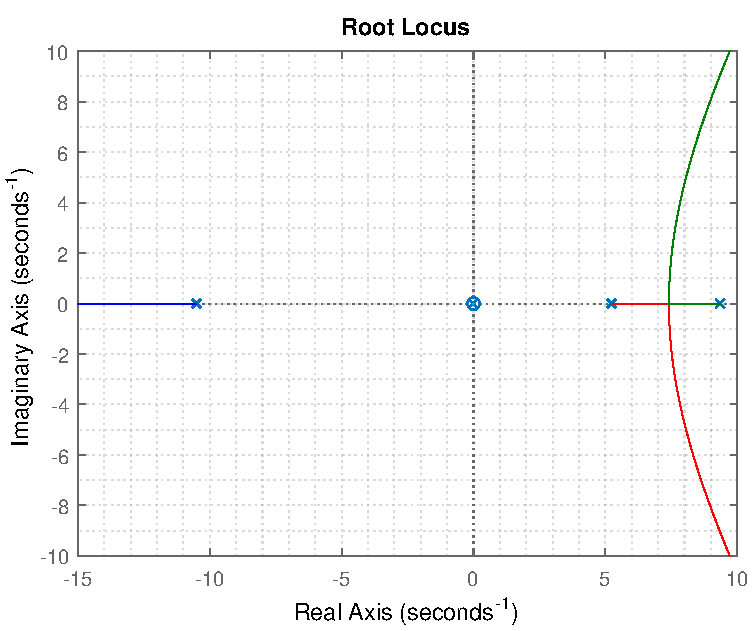
\includegraphics[scale=.55]{Pictures/RLController1}
	\centering
	\end{figure}
\end{frame}

\begin{frame}{Classical Controller Design}{Root Locus Design}	
	\begin{figure}
		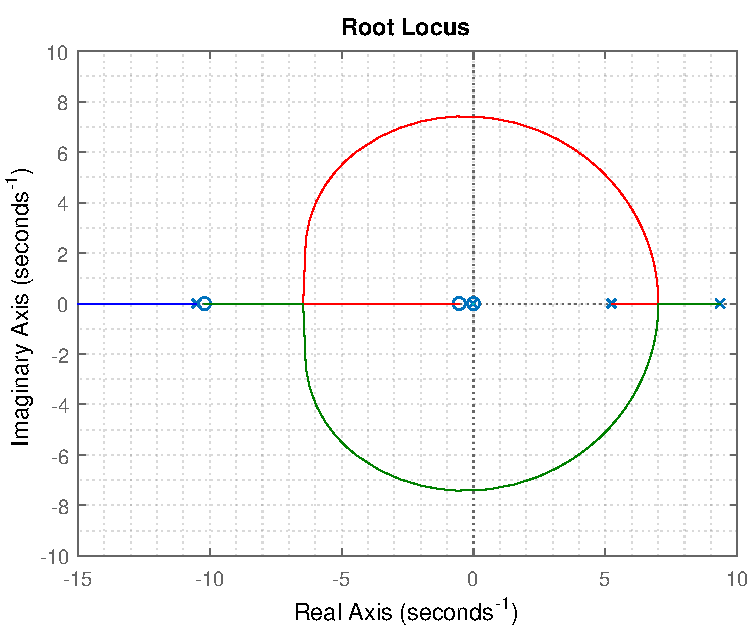
\includegraphics[scale=.55]{Pictures/RLController2}
		\centering
	\end{figure}
\end{frame}

\begin{frame}{Root Locus Designed Controller}{Root Locus Design}
\begin{figure}
	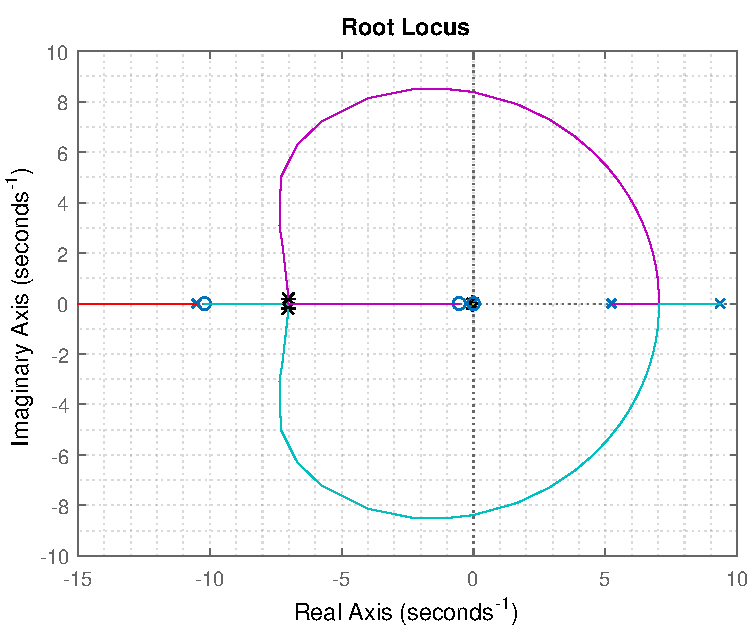
\includegraphics[scale=.55]{Pictures/RLController}
	\centering
\end{figure}	
%
\pause
%
\begin{displaymath}
	\si{D(s)\ =\ -4059,8 \cdot \frac{(s + 10,2)\cdot (s + 0,546)}{(s - 5,23) \cdot (s + 100) \cdot (s + 200)}} \nonumber
\end{displaymath}
\end{frame}

%%%%%%%%%%%%%%%%%
\subsection{Discretization}
\begin{frame}{Root Locus Designed Controller}{Discretization}	
\begin{figure}
	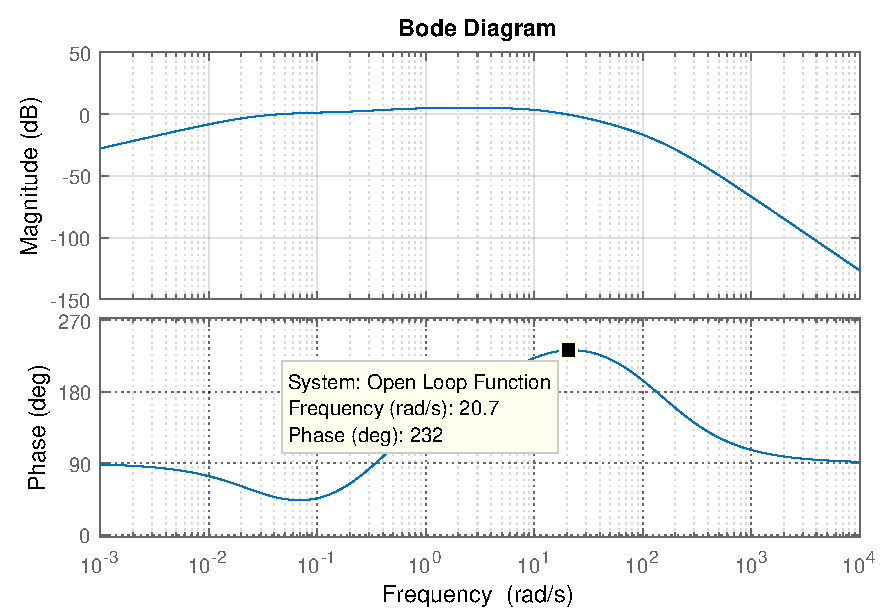
\includegraphics[scale=.543]{Pictures/bodeOL}
\end{figure}
\pause
\begin{displaymath}
	\si{D(z)\ =\ \frac{\tau_{m,w}(z)}{e_{\theta}(z)}\  = \frac{-7,338 + 6,58 \cdot z^{-1} + 7,335 \cdot z^{-2} - 6,584 \cdot z^{-3}}{1 - 1,3879 \cdot z^{-1} + 0,3409 \cdot z^{-2} + 0,001576 \cdot z^{-3}}}  \nonumber 
\end{displaymath}
\end{frame}

%%%%%%%%%%%%%%%%%
\subsection{Simulation of the Controller}
\begin{frame}{Root Locus Designed Controller}{Simulation of the Controller}
\begin{itemize}
	\item Behavior of the continuous and the discrete controllers in simulation 
\end{itemize}
\begin{minipage}{\linewidth}
	\begin{minipage}{0.45\linewidth}
		\begin{figure}
			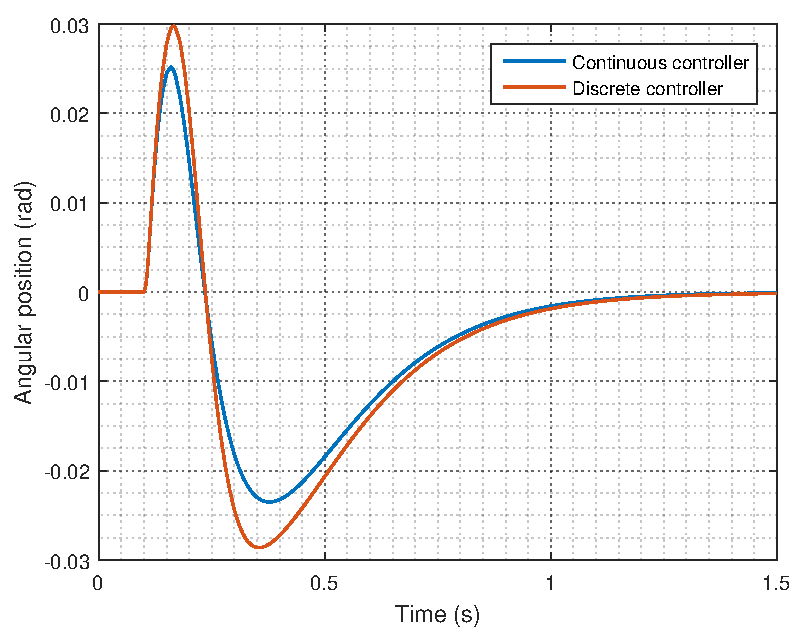
\includegraphics[scale=.37]{Pictures/positionRL}
			\centering
		\end{figure}
	\end{minipage}
	\hspace{0.05\linewidth}
	\begin{minipage}{0.45\linewidth}
		\begin{figure}[H]
			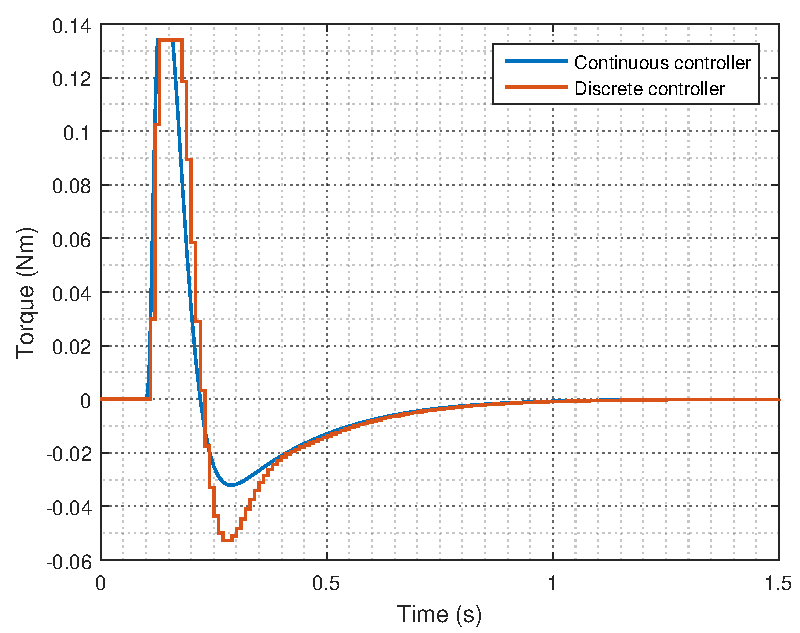
\includegraphics[scale=.37]{Pictures/torqueRL}
			\centering
		\end{figure}
	\end{minipage}
\end{minipage}
\end{frame}

%%%%%%%%%%%%%%%%%
\subsection{Implementation}
\begin{frame}{Root Locus Designed Controller}{Implementation}	
\begin{itemize}
	\item Difference equation
\end{itemize}
\begin{flalign}
  \si{\tau_{m}[n] =} & \si{\num{-8,314} \cdot e_{\theta}[n]+ \num{7,422} \cdot e_{\theta}[n-1] + \num{8,3023} \cdot e_{\theta}[n-2] }& \nonumber \\ 
   &\si{- \num{7,434} \cdot e_{\theta}[n-3] + \num{1,382} \cdot \tau_{m}[n-1] - \num{0,3415} \cdot \tau_{m}[n-2] } & \nonumber \\
   & \si{ - \num{0,001638} \cdot \tau_{m}[n-3]}& \nonumber 
\end{flalign}
\end{frame}

\begin{frame}{Root Locus Designed Controller}{Implementation}	
\begin{itemize}
	\item Angular position of the frame and angular velocity of the wheel in the real Cubli
\end{itemize}
\begin{minipage}{\linewidth}
	\begin{minipage}{0.4\linewidth}
		\begin{figure}
			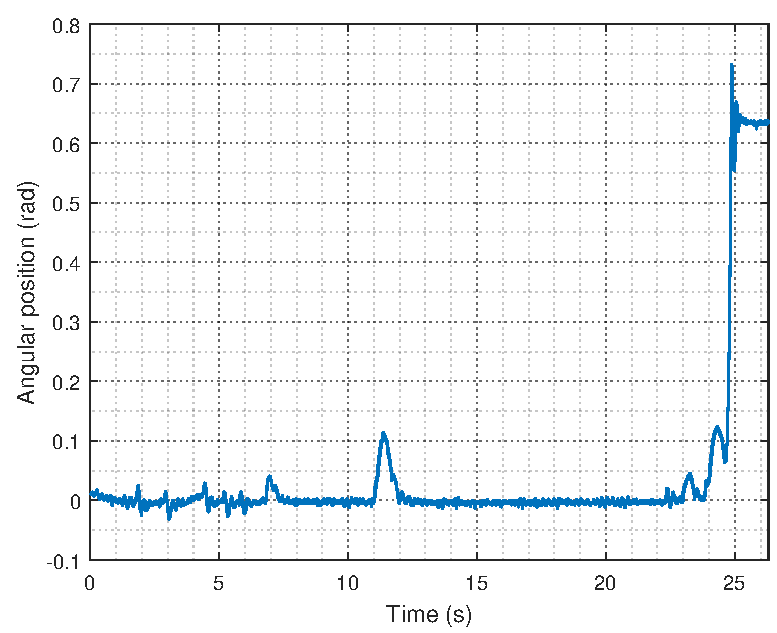
\includegraphics[scale=.35]{Pictures/positionRLTest}
			\centering
		\end{figure}
	\end{minipage}
	\hspace{0.1\linewidth}
	\begin{minipage}{0.45\linewidth}
		\begin{figure}[H]
			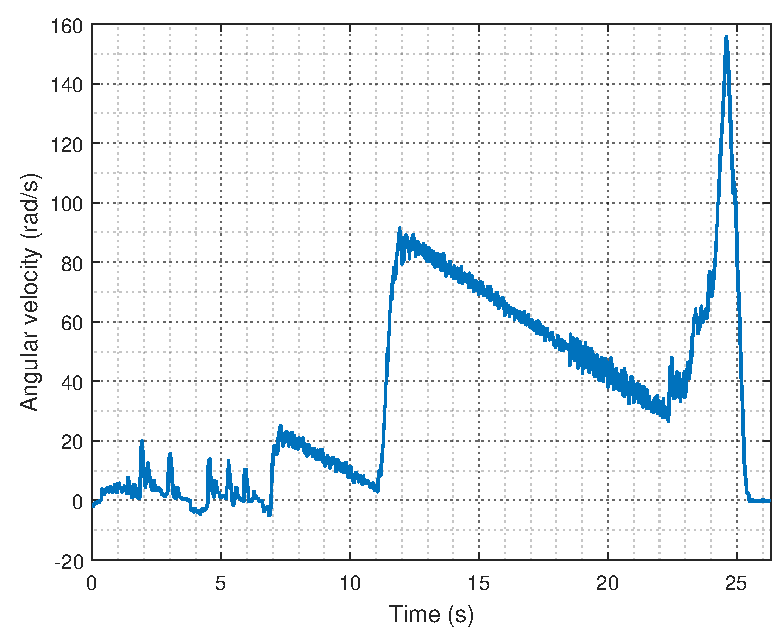
\includegraphics[scale=.35]{Pictures/wheelRLTest}
			\centering
		\end{figure}
	\end{minipage}
\end{minipage}
\end{frame}
%%%%%%%%%%%%%%%%%
